




\section{Introduction} 




\begin{frame}
    \frametitle{Linear Regression}
    We measure two variables, x and Y.

    \begin{itemize}
        \item Simple linear regression:
        \begin{itemize}
            \item How does the value of $Y$ depend on value of $x$?
            \item Is there a linear relationship?
            \item How can we estimate this relationship using observed data?
        \end{itemize}
        \item Multiple linear regression:
        \begin{itemize}
            \item We measure several vaiables $x_1,...,x_p$ and $Y$. How does the values of
            $Y$ depend on the values of $x_1,...,x_p$?
        \end{itemize}
    \end{itemize}
\end{frame}

\begin{frame}
    \frametitle{Simple Linear Regression: Example}
    \begin{figure}
        \centering
        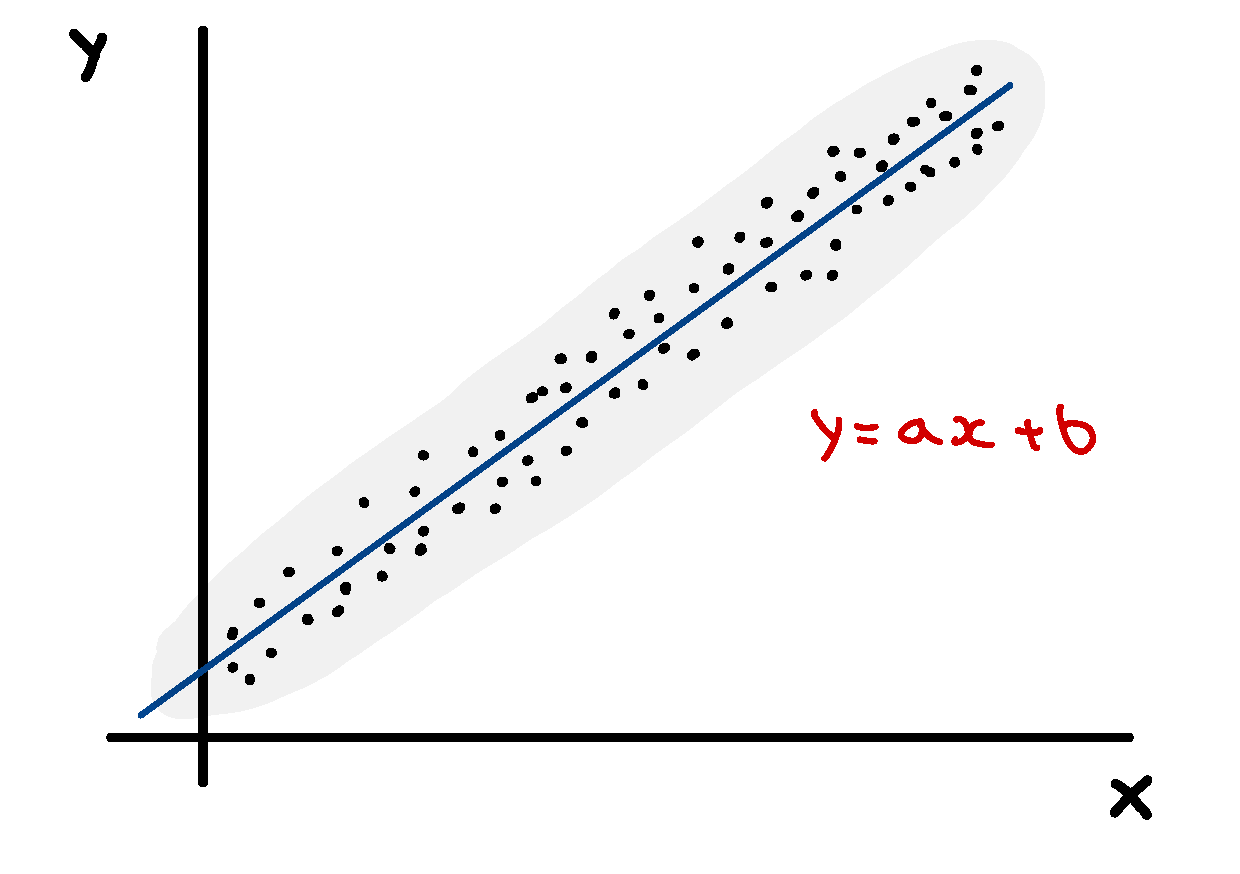
\includegraphics[width=0.95\textwidth]{sections/introduction/figures/linear_plot.pdf}
    \end{figure}
\end{frame}


\begin{frame}
    \frametitle{Basic assumptions}

    \begin{itemize}
        \item $x_1,...,x_p$: independent variables and assumed non random
        \item Y: continuous dependent variable and assumed \textbf{random};
        \item We hypothesize that $Y$ has a \textbf{linear relationship} with 
        $x_1,...,x_p$, \textbf{on average} and follows the linear model:

        $$E(Y) = \beta_0 + \beta_{1}x_1 + ... + \beta_{p}x_p$$

        \item $\beta_0,\beta_1,...,\beta_p$: unknown parameters, assumed non random
        \item $\beta_0$ = intercept (when $x_1 = ... = x_p = 0$);
        \item $\beta_1,...,\beta_p$ = slopes in the corresponding $x$-directions.
    \end{itemize}

\end{frame}


\begin{frame}
    \frametitle{Basic assumptions: Multiple linear regression}

    \begin{itemize}

        \item We denote with $Y_i$, where $i = 1,...,n$, the \textbf{$i$th observation}
        from a set of $n$ measurements of $Y$;

        \item We denote with $x_{ij}$, where $i = 1,...,n$ and $j = 1,...,p$, the
        corresponding $i$th observation of the $j$th \textbf{x-variable};

        \item The model for a generic observation $Y_i$ is:

        $$Y_i = \beta_0 + \beta_{1}x_{i1} + ... + \beta_{p}x_{ip} + \epsilon_i \Rightarrow {\color{red}\epsilon_i = Y_i - \hat{Y_i}}$$

        where $i = 1,...,n$ and $\epsilon_i$ is the measurement error which contains
        all the \textbf{random variation} not explainable by the linear model.

    \end{itemize}

\end{frame}

\begin{frame}
    \frametitle{Simple Linear Regression: Example}
    \begin{figure}
        \centering
        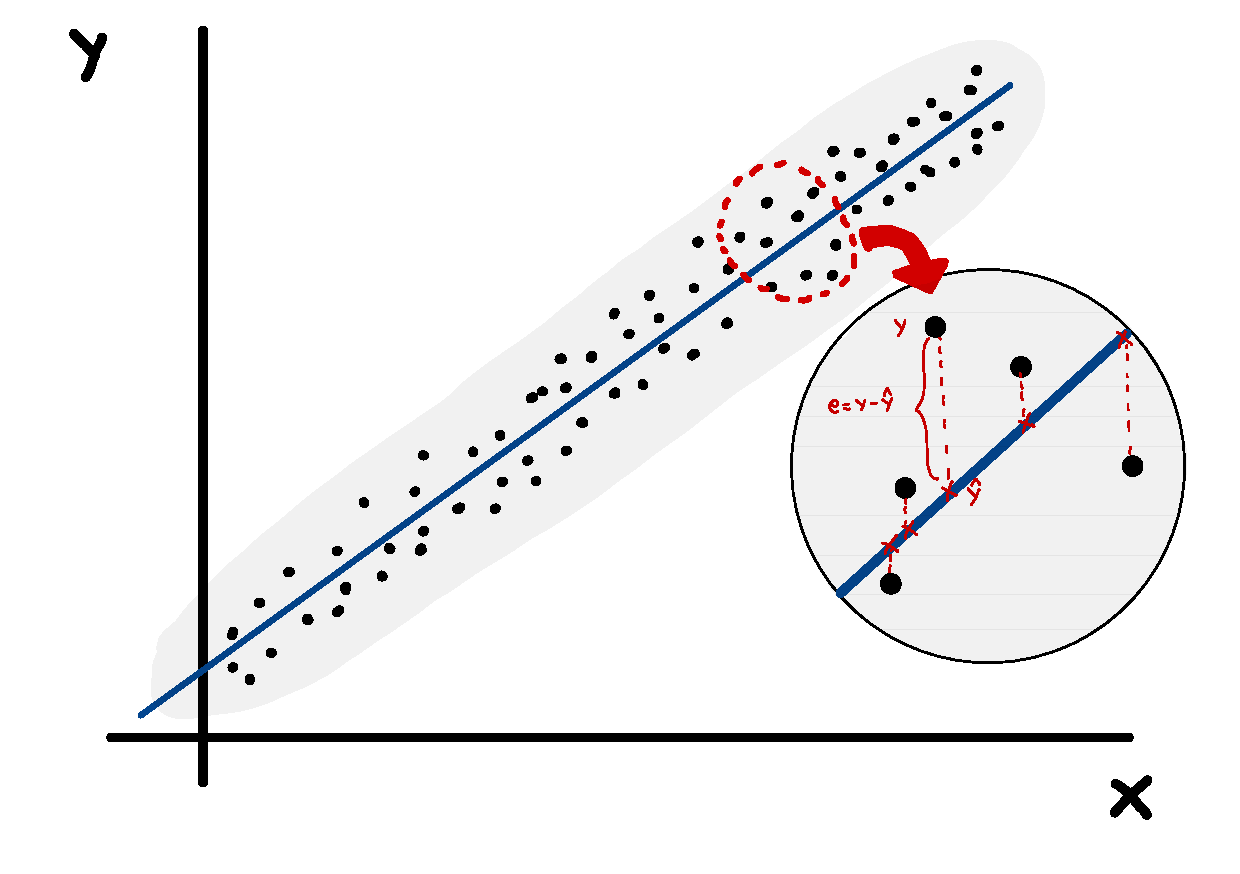
\includegraphics[width=0.95\textwidth]{sections/introduction/figures/linear_plot_with_error.pdf}
    \end{figure}
\end{frame}


\begin{frame}
    \frametitle{Multiple Linear Regression with matrices}
    \begin{figure}
        \centering
        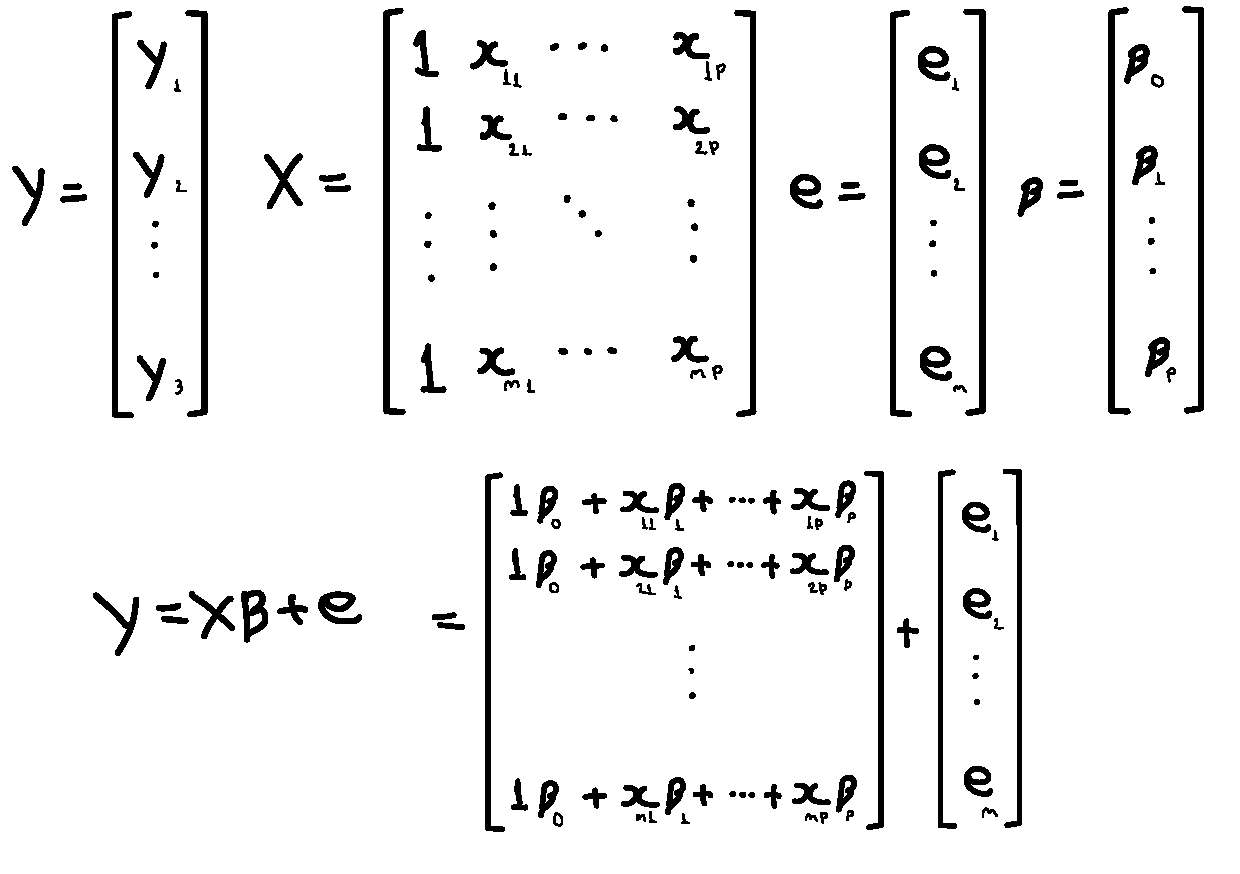
\includegraphics[width=0.95\textwidth]{sections/introduction/figures/matrix_form.pdf}
    \end{figure}
\end{frame}



\begin{frame}
    \frametitle{Basic assumptions: for the measurement error}

    Besides linearity, we also assume for all $i = 1,...,n$. 
    %Remark: $V[X]=E[(X-\overline{X})^2]$
    \begin{itemize}

        \item $\E[\epsilon_i] = \overline{\epsilon_i} = 0$
        
        \item $V[\epsilon_i] = \E[(\epsilon_i - \overline{\epsilon_i})^{2}] = \E[\epsilon_{i}^2] = \E[(Y_i-\hat{Y_i})^2] = \sigma^{2}$

        \item $\epsilon_i$ are \textbf{uncorrelated} random variables; 
        
        \item $\E[Y_i] = \E[\beta_0 + \beta_{1}x_{i1} + ... + \beta_{p}x_{ip}] + \E[\epsilon_i] = \mu_{i}$
        
        \item $V[Y_i] = V[\beta_0 + \beta_{1}x_{i1} + ... + \beta_{p}x_{ip}] + V[\epsilon_i] = \sigma^2$
    \end{itemize}



\end{frame}



\begin{frame}
    \frametitle{Multiple Linear Regression with matrices}
    \begin{figure}
        \centering
        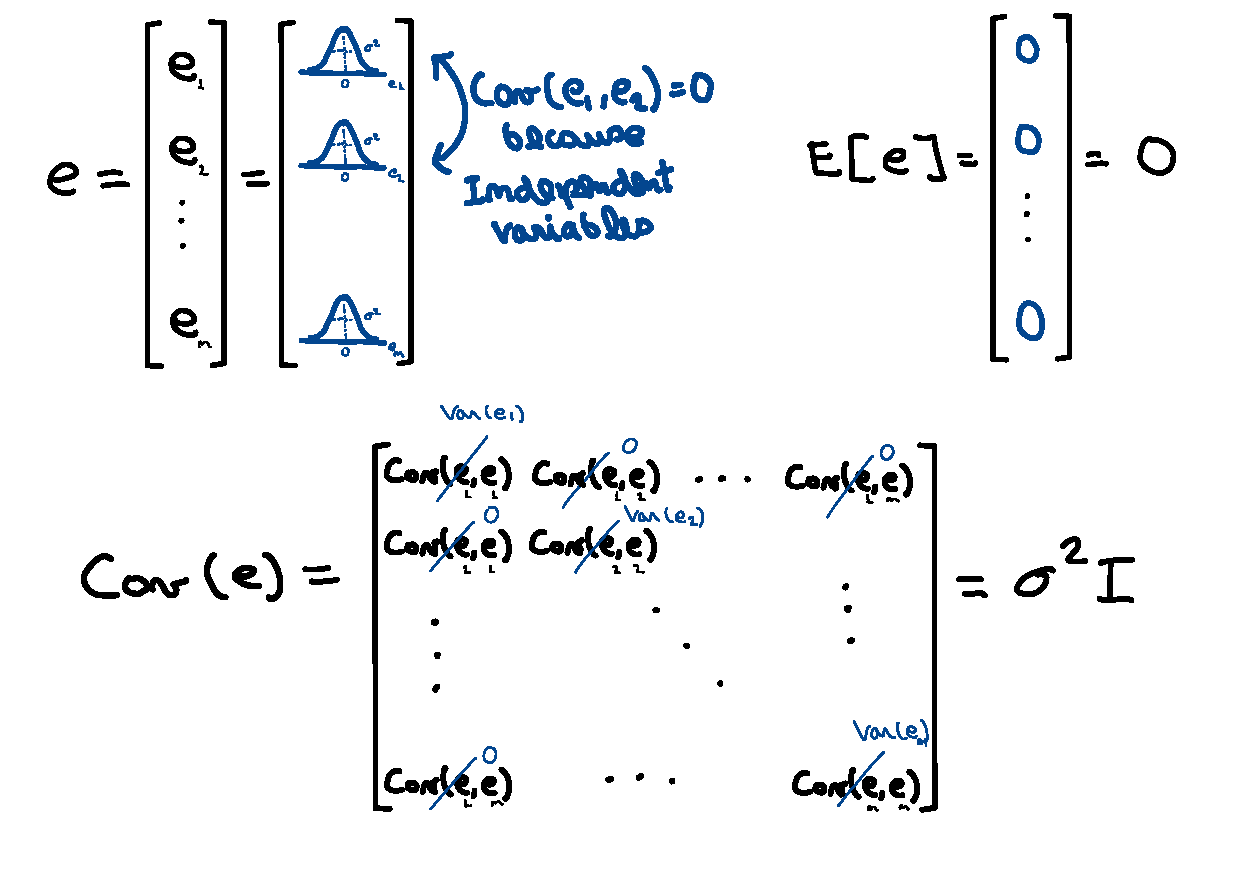
\includegraphics[width=0.95\textwidth]{sections/introduction/figures/cov_e.pdf}
    \end{figure}
\end{frame}

